\chapter{Interactions}

Following sequence diagrams only show the general idea of the algorithms used in the default implementation. This scenario show a client that access a distant object via a register connected to a naming server.

\section{Client}
\begin{figure}[H]
\begin{center}
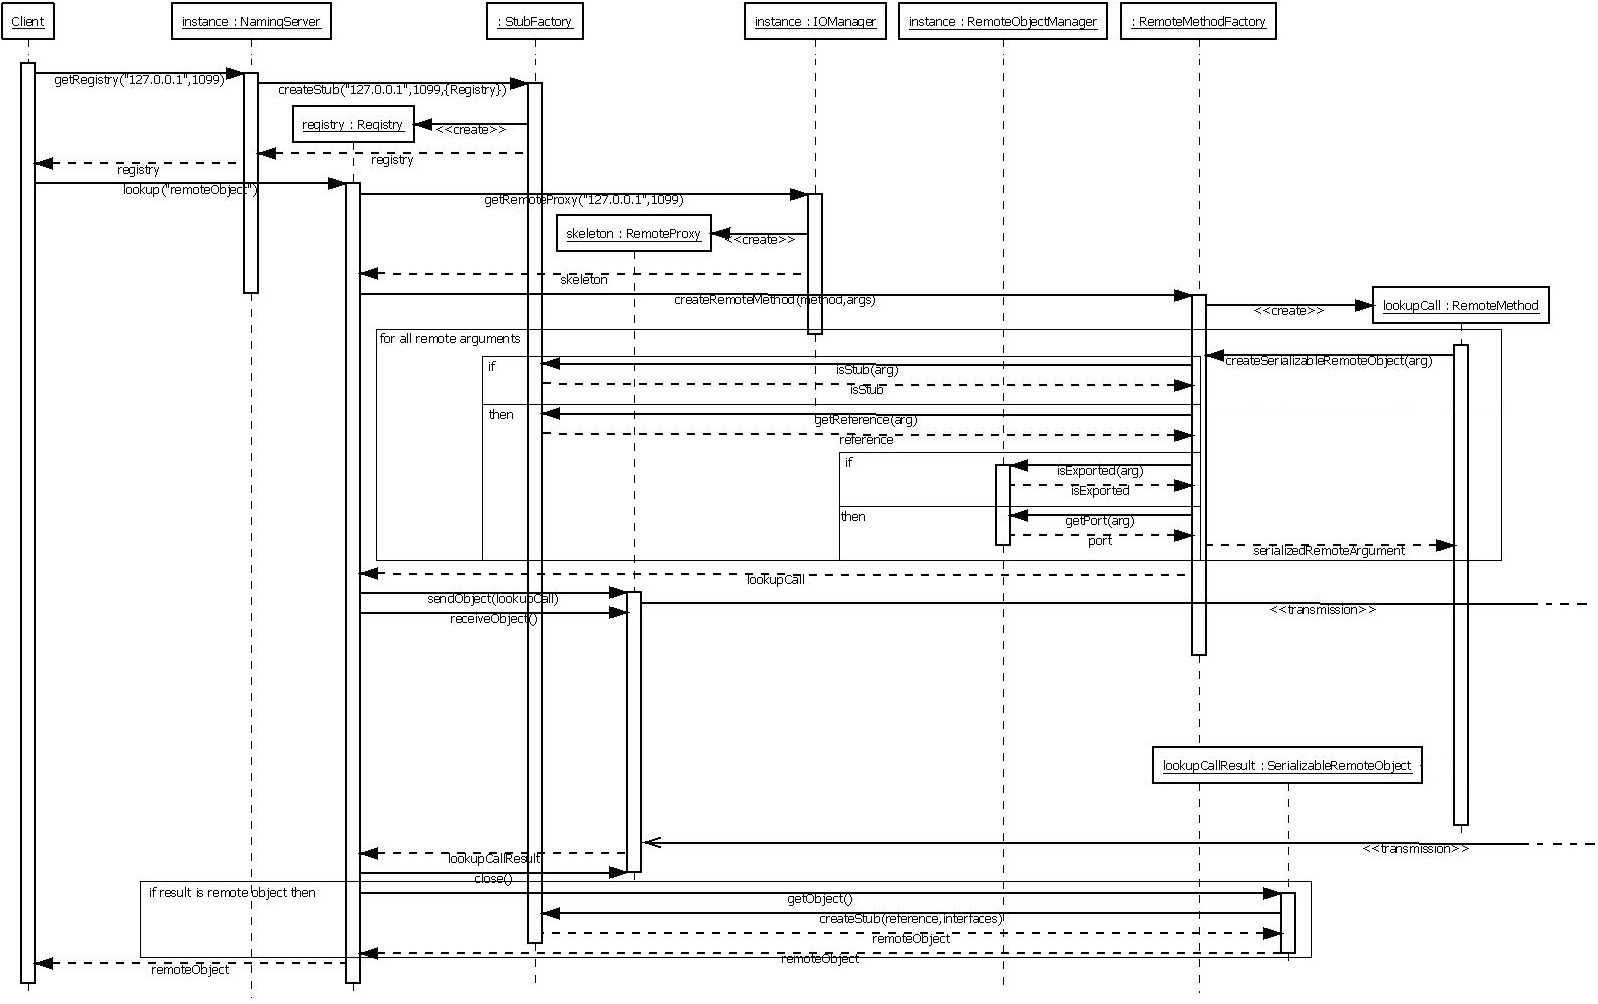
\includegraphics[scale=0.45,angle=90]{../img/diag_sequence_client.jpeg}
\caption{Sequence diagram}
\end{center}
\end{figure}
\medskip
The client gets a first stub connected to the remote registry (name server), and then retrieves an object from the server.

\section{Server}
Here, the method of createSerializableRemoteObject is simplified in order to make the diagram more readable.
\begin{figure}[H]
\begin{center}
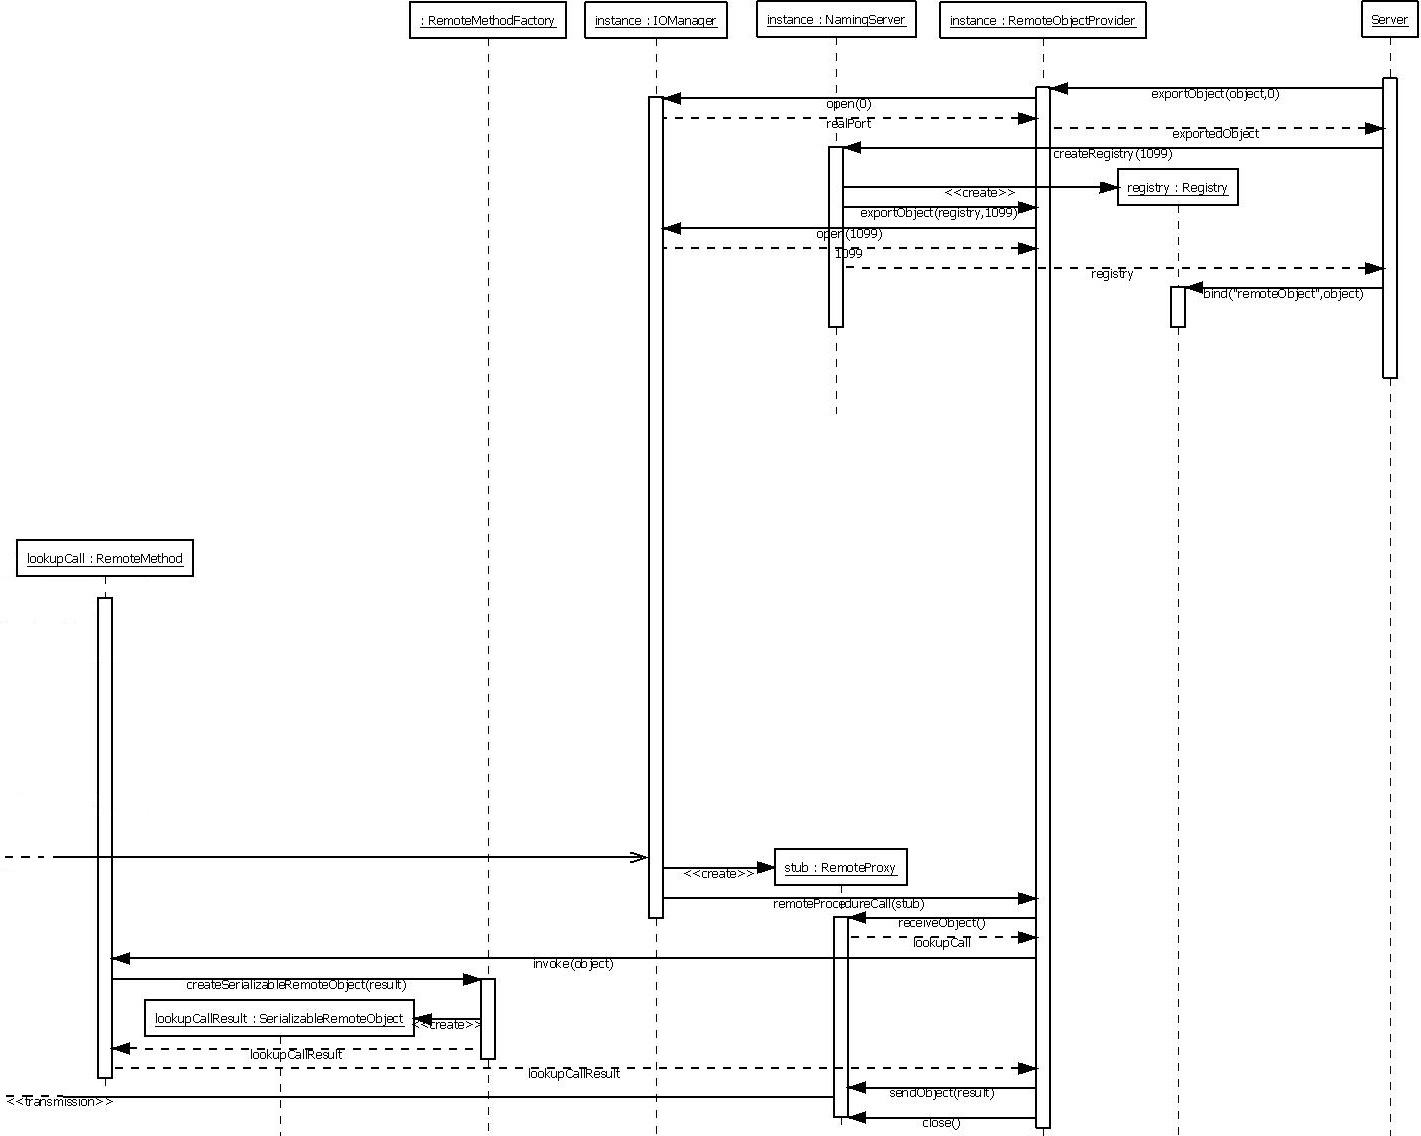
\includegraphics[scale=0.5,angle=90]{../img/diag_sequence_server.jpeg}
\caption{Sequence diagram}
\end{center}
\end{figure}

